\documentclass[conference]{IEEEtran}
%+++++++++++++++++++++++++++++++++++++++++++
% Added to commands
\input epsf
\usepackage{graphicx}
\usepackage [french]{babel}
\usepackage [utf8]{inputenc}
\usepackage [T1] {fontenc}
\usepackage{float}
\usepackage{amsmath}
%+++++++++++++++++++++++++++++++++++++++++++
% correct bad hyphenation here
\hyphenation{op-tical net-works semi-conduc-tor IEEEtran}
\begin{document}

%+++++++++++++++++++++++++++++++++++++++++++
\title{\LARGE Identification Expérimentale des Coéfficients Aérodynamiques
\vskip10pt

\small 2024 - Romain LAMBERT
}
%+++++++++++++++++++++++++++++++++++++++++++
% make the title area
\maketitle

\begin{abstract}Ce bureau d'étude a pour sujet l'identification expérimentale des coéfficients aérodynamiques. L'objectif final étant de déterminer un protocol expérimental permetant de mesurer l'angle d'incidence d'un kite; en vue d'obtenir une polaire expérimentale des voiles. 
\end{abstract}
\IEEEoverridecommandlockouts

\IEEEpeerreviewmaketitle
\section{Travaux précédents (Zoé Marcelet)}

\subsection{Modèle Lagragien} 

D'après le document \textit{"Dynamics and Control of Single-Line Kites"} de Gonzalo Sanchez-Arriaga (2006),  les formules suivantes permettent d'obtenir l'élévation $\Gamma$ et l'angle d'incidence du vent $\theta$, en fonction du vent et des coefficients aérodynamiques du kite : \\

\begin{figure}[H]
    \centering
    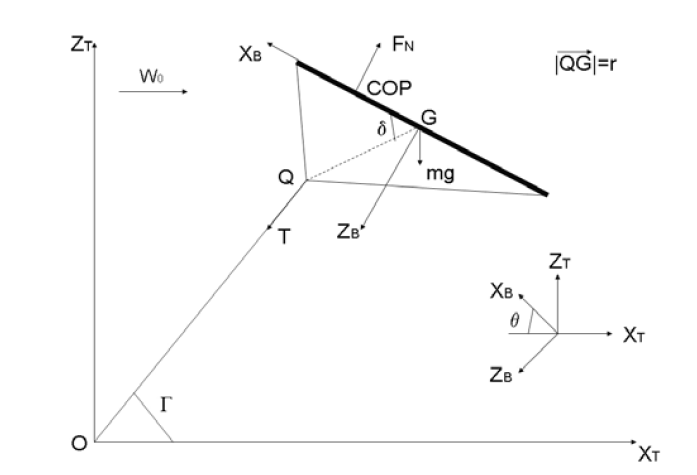
\includegraphics[width=0.5\textwidth]{Pics/Picture Sanchez.png}  
    \caption{Schéma du kite au Zénith.}
    \label{fig:sanchez}
\end{figure}

La première équation donne l’angle d’incidence $\theta$ : 
\begin{center}
    \begin{equation}
        cos(\delta - \theta) + \beta (\sigma-cos(\delta))C_N(\theta) = 0
        \label{eq:theta}
    \end{equation}
\end{center}
La deuxieme équation donne l’angle d’élévation $\Gamma$ :
\begin{center}
    \begin{equation}
        \Gamma = tan^{-1}(\frac{\beta C_N (\theta) cos(\theta)-1}{\beta C_N (\theta)sin(\theta)})
        \label{eq:gamma}
    \end{equation}
\end{center}
Avec $\beta = \frac{\rho A W_0^2}{2mg}$ et $\sigma = \frac{X_{cp}}{r}$ \\

Ces équations ont été codées (disponible sur Nextcloud : 06-RESSOURCE/AC-Admin Commun/4-Rapports Stagiaires/Stage Zoé Marcelet/Rapport\_zozo/06\_Topic\_modèle\_aéro\_zenith). \\
\textbf{Elles restent cependant peut concluantes car requièrent les coéfficients aérodynamiques du kite. }

\IEEEpeerreviewmaketitle
\section{Mesure de l'angle d'incidence au Zénith}

\subsection{Problème de l'angle de calage $\alpha_0$} 


Une première intuition nous amène à penser que la connaissance de l'angle d'élévation et de la géométrie des bridages permet de remonter à l'angle d'incidence $\alpha$

\begin{figure}[H]
    \centering
    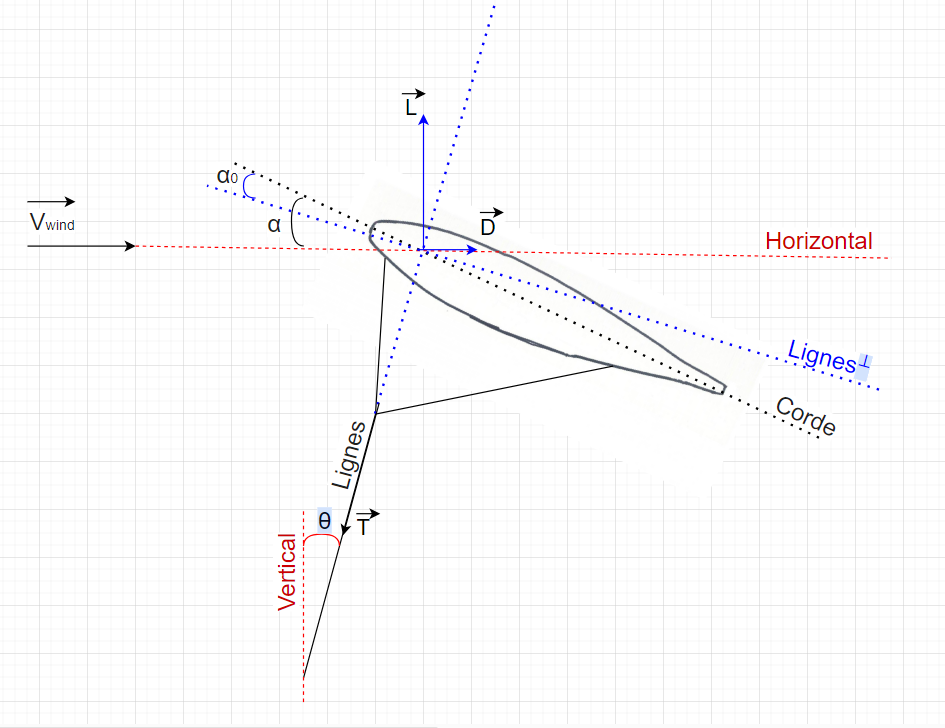
\includegraphics[width=0.5\textwidth]{Pics/Schéma Equilibre Zéntih.png}  
    \caption{Schéma des angles qui paramètres le Zénith.}
    \label{fig:Zénith alpha zéro}
\end{figure}

La figure \ref{fig:Zénith alpha zéro}, l'angle $\alpha_0$ dépend de considération aérodynamique, car : 
\begin{center}
    \begin{equation}
        \frac{L}{D} = \frac{1}{tan(\theta)} = \frac{1}{tan(\alpha + \alpha_0)}
    \end{equation}
\end{center}
Ainsi, l'angle que fait le cône de bridage avec les lignes qui le relient au sol s'adapte (via l'angle $\alpha_0$) de sorte à aligner les efforts aérodynamiques avec les lignes des avants. Ainsi, cette angle permet de lier "géométrie" et "aérodynamique" :  

\begin{figure}[H]
    \centering
    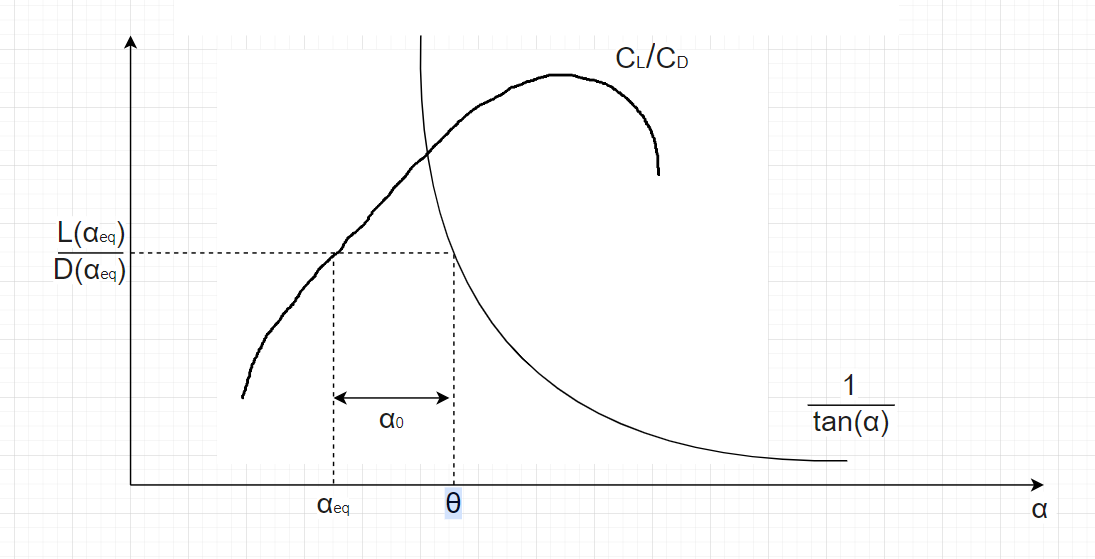
\includegraphics[width=0.5\textwidth]{Pics/Schéma Equilibre finesse.png}  
    \caption{Graphique du lien entre finesse (aérodynamique) et l'angle $\alpha_0$}
    \label{fig:Zénith finesse}
\end{figure}

\textbf{Cependant,} la formule à l'équilibre suivante (voir "equilibre kite" pour demo) : 

\begin{center}
    \begin{equation}
        x_T = \frac{L x_F - P x_G -C_{M_0}}{L - P}
    \end{equation}
\end{center}

montre qu'en \textbf{vent fort}, pour $C_{M_0} = 0$, $x_T = x_F$, et donc on peut déterminer géométriquement $\alpha_0$ ! \textbf{Donc la mesure de l'angle $\theta$ permet de remonter à $\alpha$ et à la finesse $\frac{L}{D}$}

\subsection{Utiliser un capteur de tension pour les A et les B au niveau du kite}
\label{sec:tension AB}

L'idée est que notre système \{kite+bridages\} se comporte comme un pendule inversé. Mesurer les tensions dans les A et les B permet de mesurer la position de la résultante aérodynamique le long du kite et ainsi de prédire son angle d'incidence $\alpha$ en s'affranchissant de la polaire aérodynamique du kite. 

\begin{figure}[H]
    \centering
    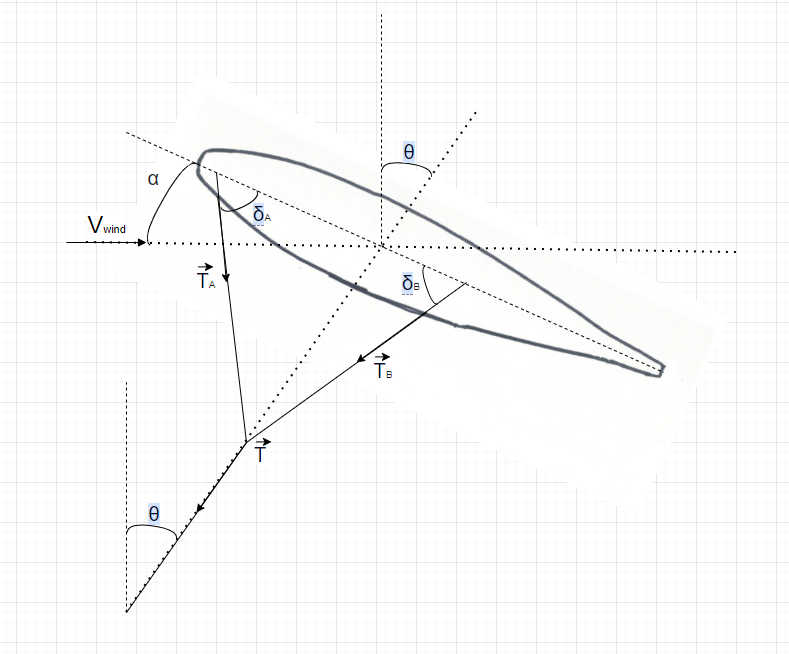
\includegraphics[width=0.5\textwidth]{Pics/Schéma Equilibre capteurs tension AB.png}  
    \caption{Schéma des tensions dans les bridages}
    \label{fig:Zénith tensions AB}
\end{figure}

Le graphe \ref{fig:Zénith tensions AB} permet d'écrire la relation suivante : 
\begin{center}
    \begin{equation}
        T_A cos(\delta_A) - T_B cos(\delta_B) = T cos(\frac{\pi}{2} +\alpha - \theta)
    \end{equation}
\end{center}

et ainsi d'en déduire :

\begin{center}
    \begin{equation}
        \alpha = \theta + sin^{-1}(\frac{T_B cos(\delta_B) - T_A cos(\delta_A)}{T}))
        \label{eq:alpha}
    \end{equation}
\end{center}

Ainsi, on peut déterminer l'angle d'incidence $\alpha$ à partir de :
\begin{itemize}
    \item T : la tension des avants ( capteur "3 axes" )
    \item $\theta$ : $\frac{\pi}{2}$ - l'angle d'élévation (capteur "IMU")
    \item $T_A$ : la tension dans les A au point d'attache du kite (capteur "cyclops")
    \item $T_B$ : la tension dans les B au point d'attache du kite (capteur "cyclops")
    \item $\delta_A$ : l'angle des A par rapport à la corde moyenne du kite (surfplan ou au laser)
    \item $\delta_B$ : l'angle des B par rapport à la corde moyenne du kite (surfplan ou au laser)
\end{itemize}

\subsection{La sonde pitot}
L'équilibre au Zéntih permet d'obtenir : 

\begin{equation}
    \begin{cases}
        L = P + T sin(\theta) \\
        D = T cos(\theta) \\
        0 = C_{M_0} + (x_T - x_F) (L cos(\alpha) + D sin(\alpha)) - P cos(\alpha) (x_T - x_G)
    \end{cases}
    \label{eq:equilibre aero}
\end{equation}


Ainsi, couplé avec les résultats du chapitre \ref{sec:tension AB}, on peut mesure $L(\alpha), D(\alpha)$ et $\alpha$ à partir des capteurs cités dans ce même chapitre. 
Cependant, la connaissance du vent en altitude, à 50m de haut, est incertaine et l'ajout de la sonde pitot, fixée à un kite stable, permet d'obtenir avec précision les coéfficients $SC_L$ et $SC_D$ via :

\begin{equation}
    \begin{cases}
        L = \frac{1}{2} \rho V^2 SC_L \\
        D = \frac{1}{2} \rho V^2 SC_D 
    \end{cases}
    \label{eq:clcd}
\end{equation}

Les modèles de couches limites sont de la forme 
\begin{equation}
        u(z) = -C \mu e^{\frac{z}{\lambda}} sin(\frac{z}{\lambda}) \\
\end{equation}

où les différents coéfficients sont charactéristiques du lieu. (\textbf{Source :} \textit{Sébastien Blein. Observation et modélisation de couche limite atmosphérique stable en relief complexe : le processus turbulent d’écoulement catabatique. Météorologie. Université Grenoble Alpes, 2016. Français. ffNNT : 2016GREAI023ff. fftel-01622676f} - équation 2.69 du chapitre 2.3.1 (modèle de Prandtl)). \\

\textbf{Ainsi, on propose de mesurer les vitesses à différentes hauteurs grâce à la sonde pitot afin d'établir un modèle de couche limite pour un lieu (\textit{plage de Pereire}) et une provenance de vent (\textit{Nord-Ouest-Sud}) [l'état. de la couche limite dépend des obstacles qui précèdent le lieu de mesure]}

\subsection{Conclusion }

Muni des capteurs
\begin{itemize}
    \item 3 axes
    \item IMU
    \item Cyclops
    \item Sonde pitot\\
\end{itemize} 

On propose de :
\begin{itemize}
    \item Mesurer $\alpha$ grace à l'équation \ref{eq:alpha}, et le couple $(L(\alpha);D(\alpha))$ grace à l'équation \ref{eq:equilibre aero}. Répéter l'essai pour différentes valeurs de \textbf{TowPoint}
    \item Déterminer un modèle de couche limite grâce à la sonde pitot en mesurant des valeurs de vitesse vent à différentes hauteurs (\textit{réunion avec Delft mercredi 16/10 et voir avec mecatro pour filtrer/moyenner mesures})
    \item Déduire grâce à \ref{eq:clcd} les coéfficients aéro au zénith.
\end{itemize} 


\end{document}